\section{Nuovo Sportello}

In questa sezione descriverò in modo dettagliato le parti dell'infrastruttura che ho esplorato durante il tirocinio e che ho approfondito grazie al lavoro svolto.

\subsection{Formazione e descrizione di Nuovo Sportello}

Nel primo periodo c'è stato naturalmente un periodo di formazione, svolto in presenza nella sede di Padova di Lynx. \\ 
pdfDurante le ore di formazione, il tutor \NST mi ha presentato l'architettura di Sportello in ogni sua parte, con le tecnologie utilizzate. Ho avuto modo di entrare in contatto per la prima volta con un sistema molto complesso e di vederne la sua evoluzione nel tempo. \\

\begin{figure}[!ht]
    \centering
	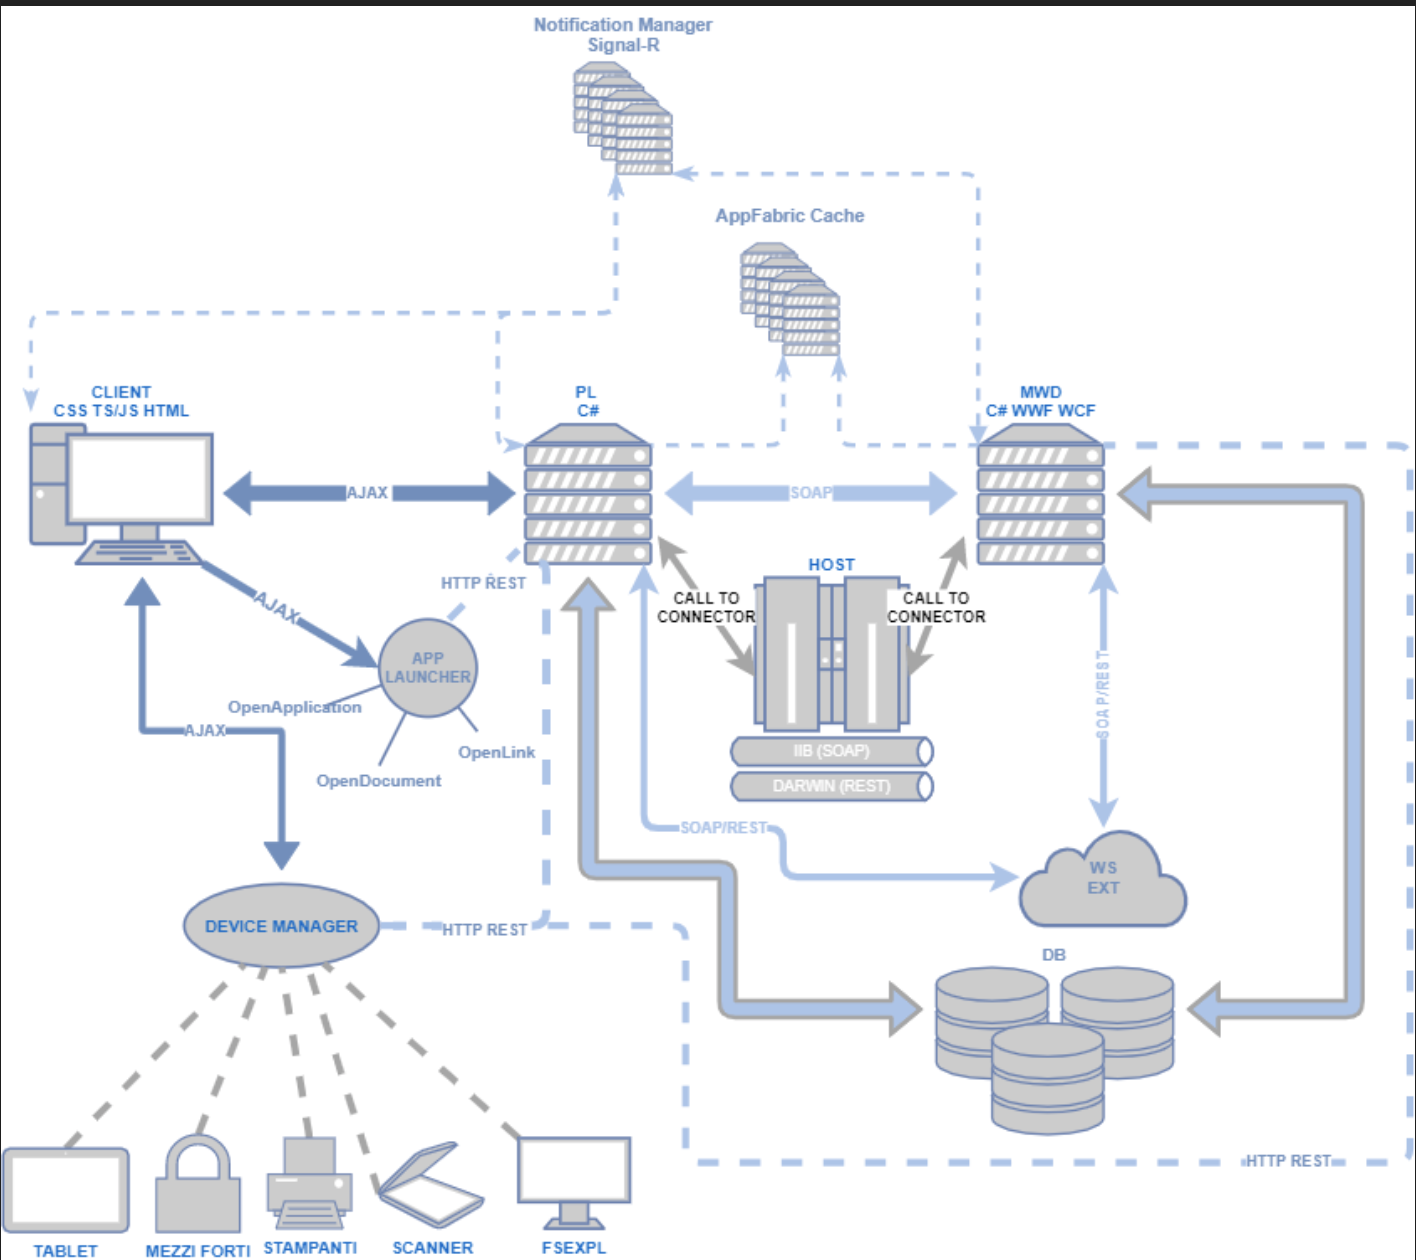
\includegraphics[width=0.85\textwidth]{./res/img/infrastruttura sportello.png}
    \caption{Overview dell'infrastruttura di Sportello}
\end{figure}

Com'è possibile vedere dalla figura la parte front-end dell'infrastruttura a sinistra è basata su ASP.NET. Il client scritto in Typescript e HTML comunica tramite chiamate Ajax con un server chiamato Presentation Layer scritto in C\#, il quale contiene tutta la logica complessa e ha la possibilità di eseguire chiamate ai server di Intesa SanPaolo o a collegarsi a servizi Middleware. Questa parte è responsabile anche del collegamento a device fisici controllabili via software. \\
Nel back-end ho già nominato i server Middleware che si occupano di esporre servizi basati su protocolli di tipo SOAP. In questo frangente sono venuto a contatto con una tecnologia Microsoft: \textit{WCF}. Windows Communication Foundation (WCF) è un framework per costruire servizi in modo sicuro ed è efficiente. È utilizzata anche una versione Event Driven con una programmazione grafica, attraverso file .xaml, chiamata Windows Workflow Foundation. \\
Sempre a back-end sono disponibili tutti i DB basati su Microsoft SQL Server e l'host di Intesa SanPaolo, server contente tutti i dati della banca. 

\subsection{Ambienti di Sportello}

Sportello viene sviluppato testato e rilasciato in 3 ambienti diversi, chiamati: \textbf{SVIL}, \textbf{UAT} e \textbf{SYSTEM}.

\subsubsection{SVIL}

L'ambiente di sviluppo é il primo in cui vengono rilasciate le modifiche a Sportello. Qui gli sviluppatori su richiesta possono chiedere una build (tramite RTC, il sistema di versioning utilizzato) e testare l'applicazione eseguendo debugging da browser, per esempio. Come visibile in figura é facile notare che le stesse componenti dell'infrastruttura di sportallo sono replicate all'interno dell'ambiente. Si può notare che SVIL possiede un proprio DB che mantiene anche le proprie configurazioni, oltre ad avere accesso ai database di SYSTEM, in produzione. \\
É presente in realtà un altro ambiente utilizzato soprattutto in per interventi per ticket con altra priorità. Questo ambiente chiamato \textbf{BFIX} é mantenuto sempre allineato con SYSTEM, in modo tale da risolvere problemi importanti che sono presenti in produzione e rilasciarli il più velocemente possibile. 


\begin{figure}[!ht]
    \centering
	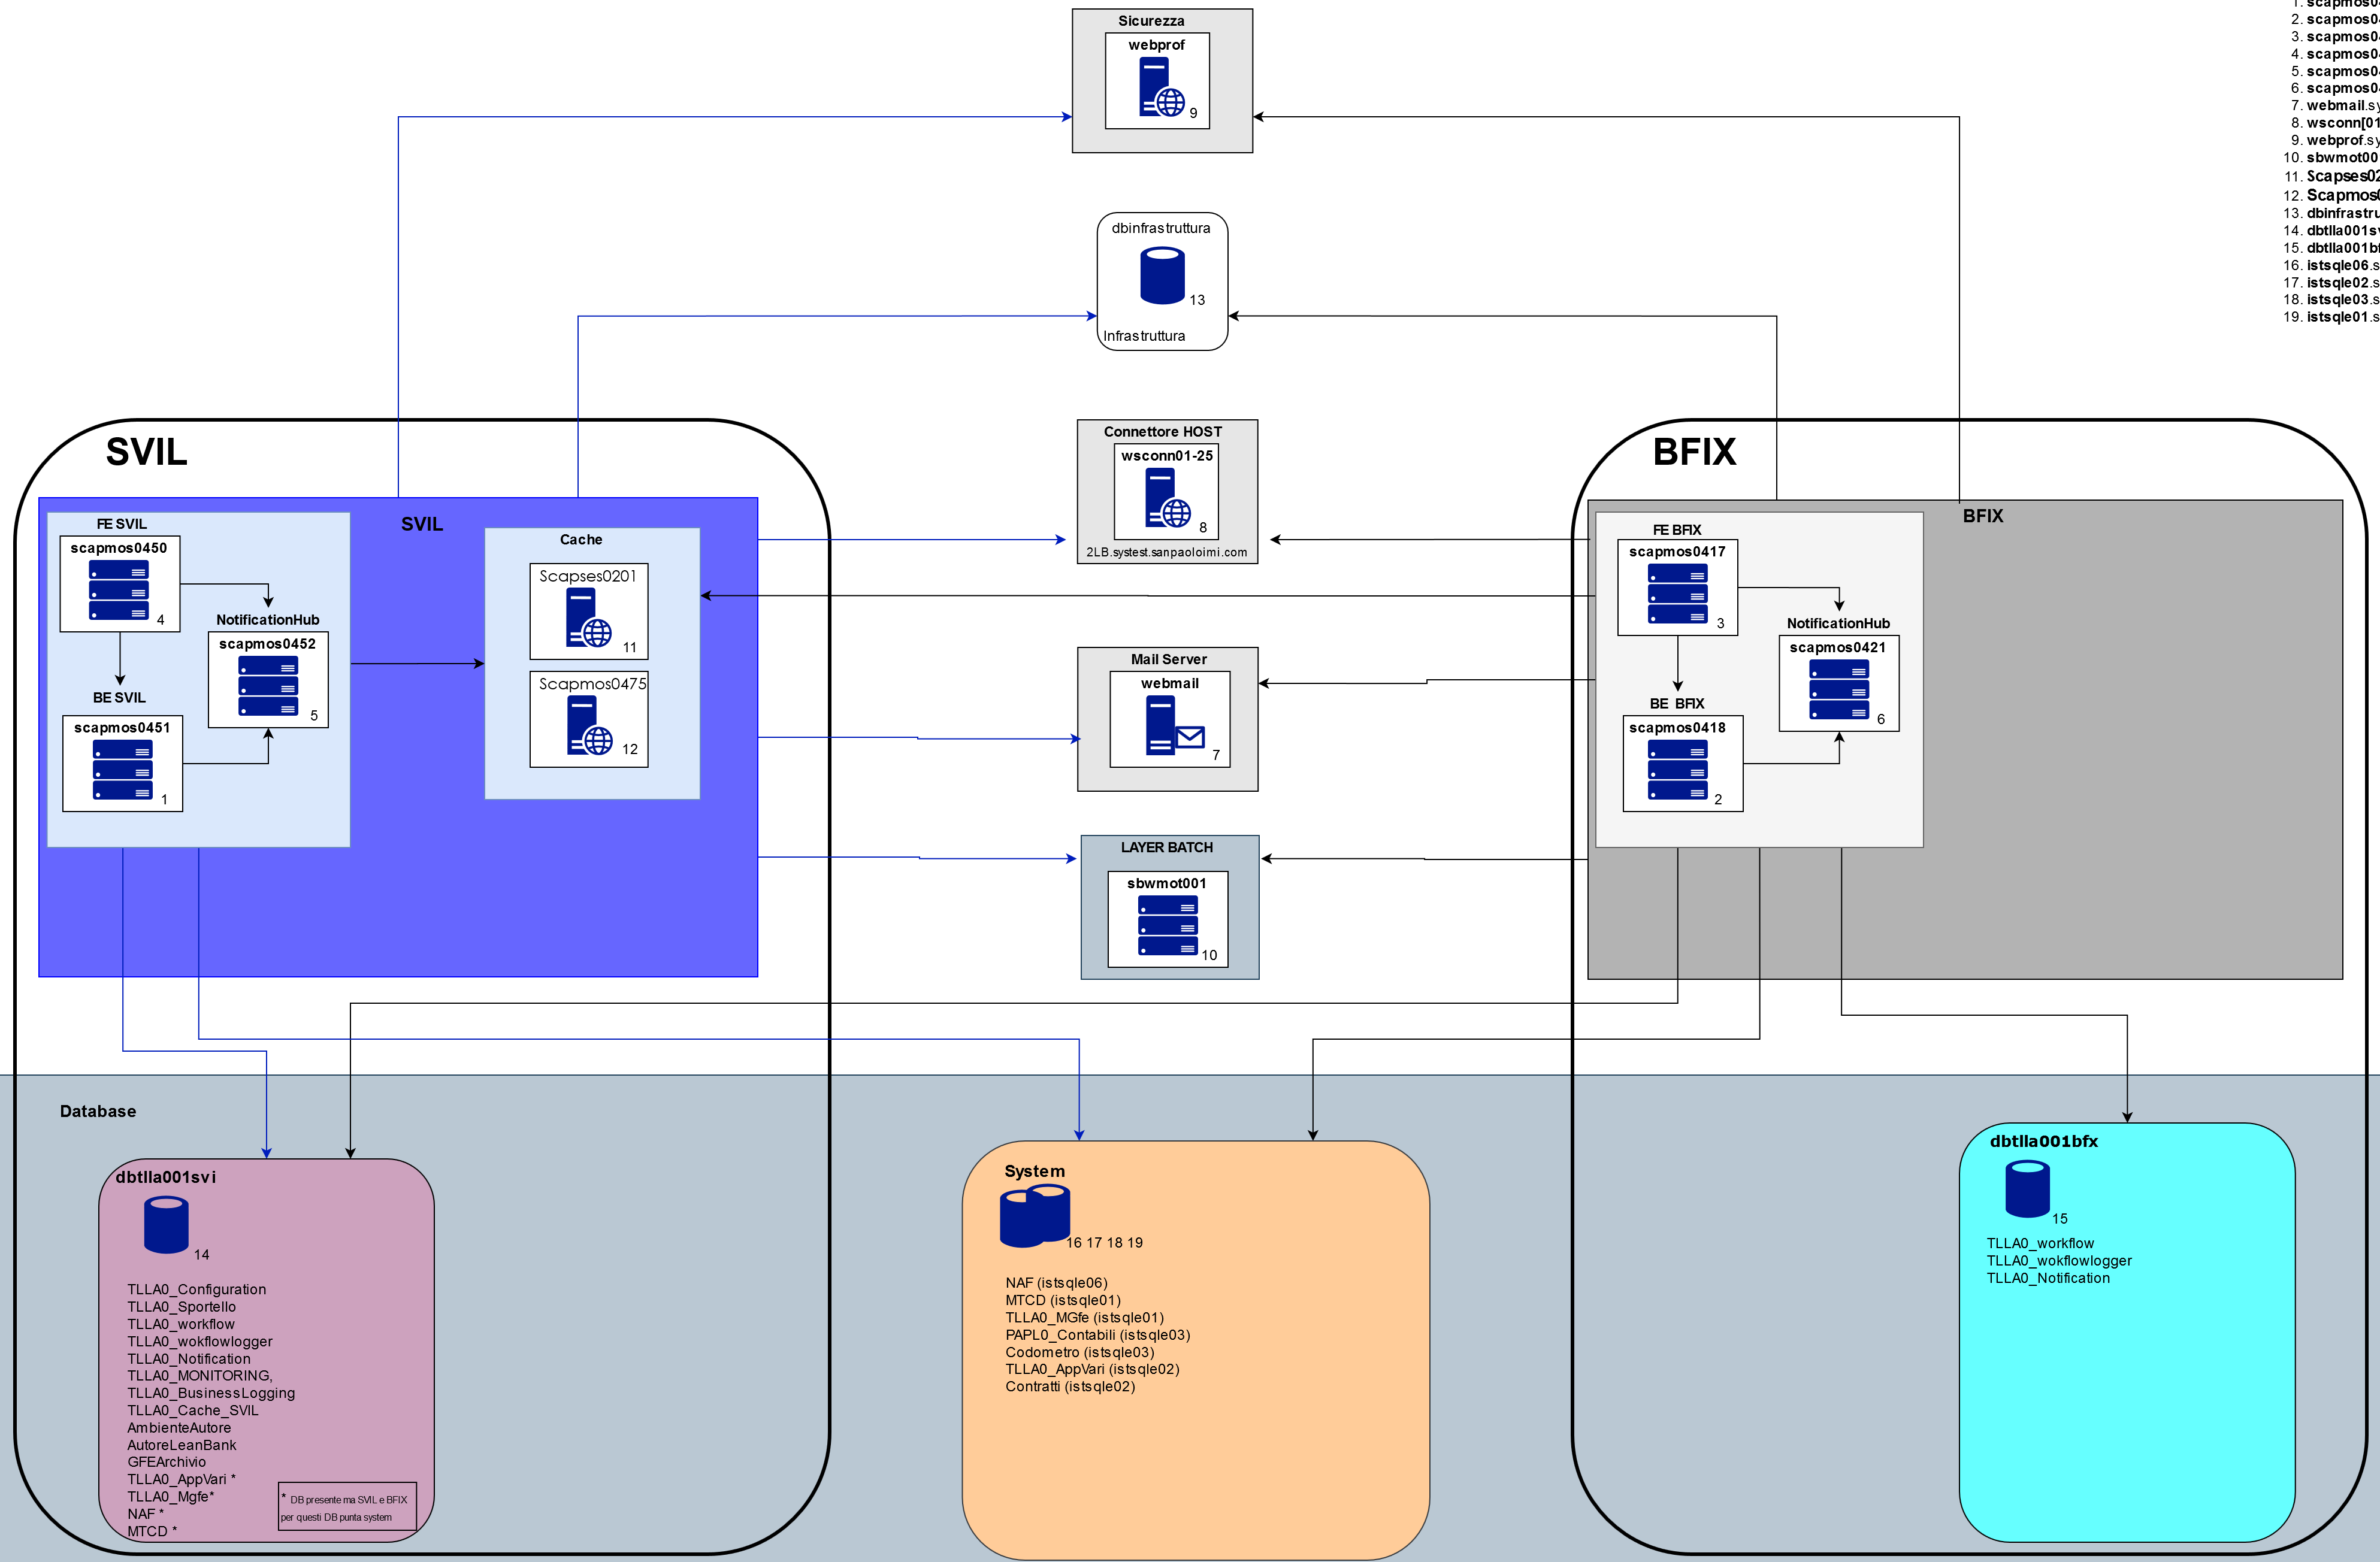
\includegraphics[width=0.85\textwidth]{./res/img/svil-diag.png}
    \caption{Overview dell'infrastruttura dell'ambiente SVIL}
\end{figure}

\subsubsection{UAT}

L'ambiente UAT é predisposto per il testing da parte di un team predisposto dal cliente. Qui alcuni dipendenti predisposti di Intesa testano le modifiche più importanti o il rilascio di nuove funzionalità. Su UAT si trova una versione successiva rispetto a quella presente in produzione. Se il software passa i requisiti imposti dal cliente, può essere rilasciato in SYSTEM.

\begin{comment}
\begin{figure}[!ht]
    \centering
	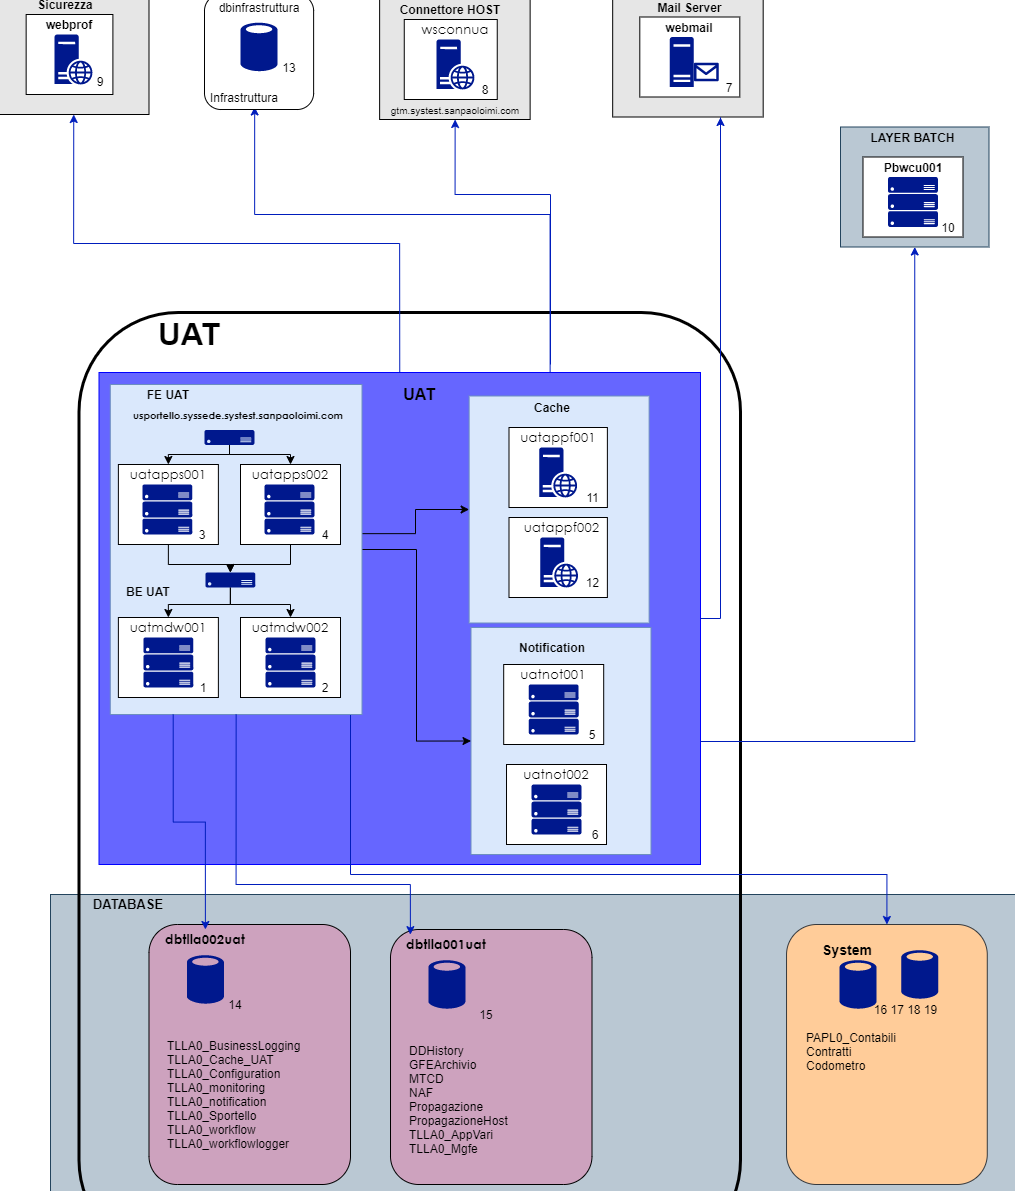
\includegraphics[width=0.75\textwidth]{./res/img/Collegamenti_UAT.png}
    \caption{Overview dell'infrastruttura dell'ambiente UAT}
\end{figure}
\end{comment}

\subsubsection{SYSTEM}

SYSTEM é l'ambiente di produzione. Qui esiste solo codice verificato e testato. Inoltre il sistema é costantemente monitorato sia dal cliente che da Lynx stessa.  \\
Si può notare dallo schema che i server stessi sono localizzati in punti geografici diversi, ma hanno lo stesso punto di accesso e gli stessi collegamenti alle altre componenti. \\
Solitamente le modifiche approvate in \textit{UAT} o che riguardano grosse componenti, escono in alcune filiali di prova filtrate tramite cosiddette \textit{chiavi di rollout}.  

\begin{figure}[!ht]
    \centering
	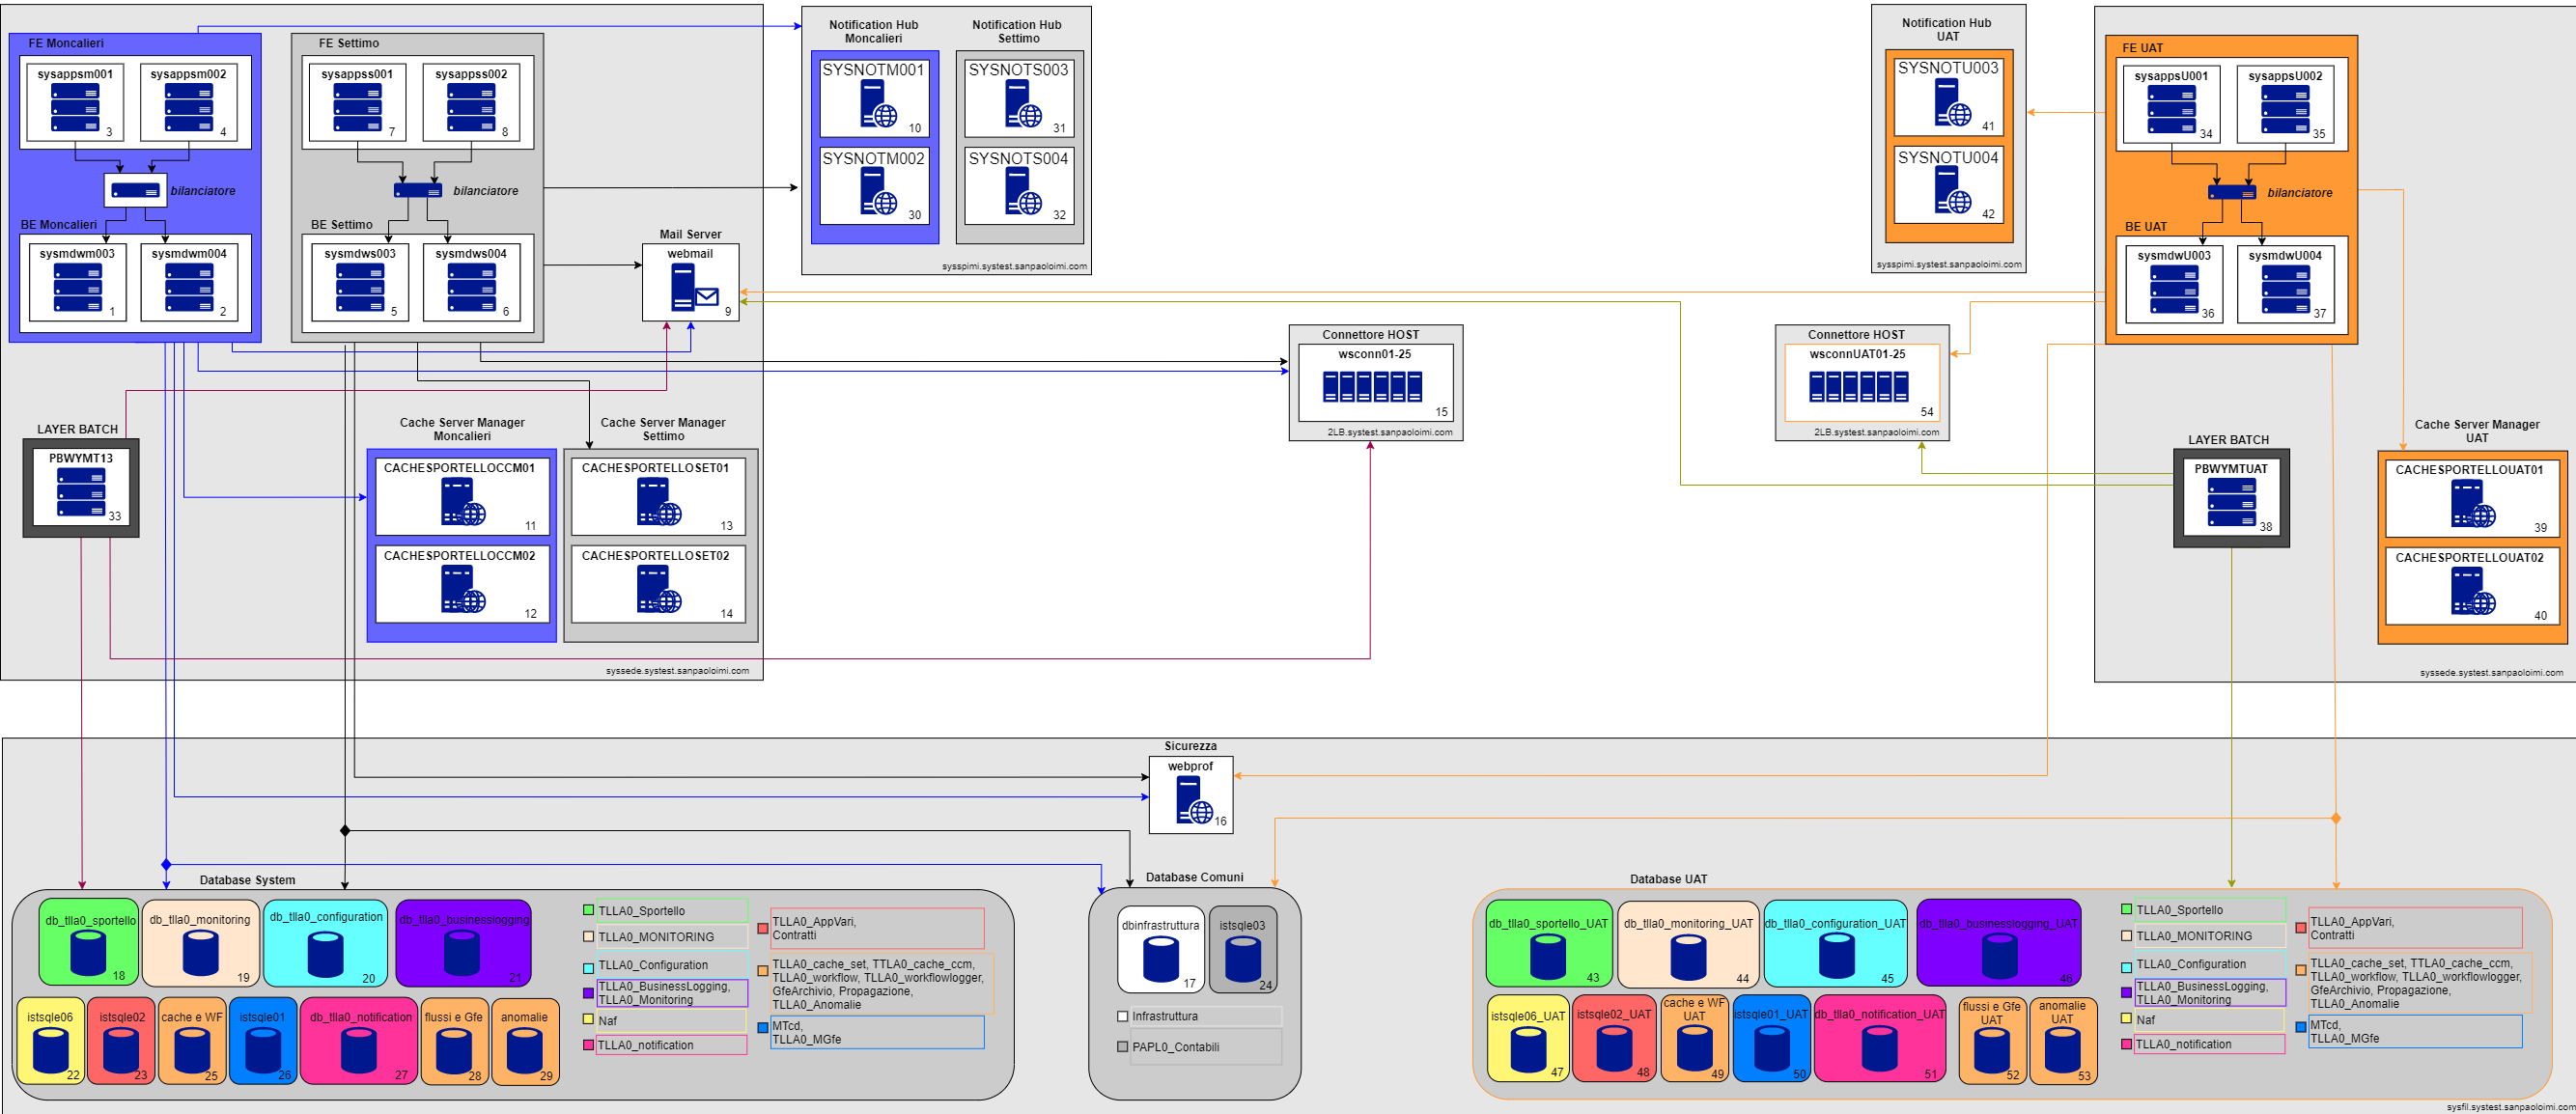
\includegraphics[width=0.85\textwidth]{./res/img/SchemiAmbienti_SYSTEM-UAT_v1.1.png}
    \caption{Overview dell'infrastruttura dell'ambiente SYSTEM e UAT}
\end{figure}

\subsection{Tecnologie utilizzate}

\subsubsection{ASP.NET}
ASP.NET è un framework creato da Microsoft per lo sviluppo di web application. Segue il pattern MVC (Model View Controller), ripreso poi dall'infrastruttura front end di Sportello. La view è costruita attraverso le normali tecnologie web, mentre il model e il controller sono scritti in C\#. I model non sono nient'altro che \textit{contract} che vengono utilizzati nel comunicazioni Ajax tra le componenti. I controller espongono metodi utili al front end implementandone la logica di fondo.  

\subsubsection{KnockoutJS}

\subsubsection{Ajax}

\subsubsection{SOAP}
Durante la prima fase del tirocinio mi è stato molto utile il concetto di chiamata SOAP. Il \textit{Simple Object Access Protocol} è utilizzato per scambiare informazioni strutturate basato principalmente su HTTP. SOAP utilizza un sistema di incapsulamento delle informazioni e anche per questo è portato per il trasporto di oggetti.

\subsection{Strumenti utilizzati}

\subsubsection{Visual Studio 2013/2017}
\begin{wrapfigure}{R}{0.25\textwidth}
    \begin{center}
        
\includegraphics[width=0.15\textwidth]{./res/img/visual-studio-2013-logo.png}
        \caption{Logo di Visual Studio}
    \end{center}
\end{wrapfigure}

L'IDE principale utilizzato durante lo sviluppo é stato naturalmente Visual Studio. Integrato nativamente con il framework ASP.NET e il linguaggio C\#, non é stato di difficile utilizzo. \\ É disponibile un interfaccia per la gestione dei pacchetti e delle librerie esterne tramite \textbf{NuGet}. É stato interessante gestire e integrare le varie \textbf{.dll} (estensione delle librerie Windows). \\ É ovviamente presente uno strumento per la build automatica e uno per il testing. \\
Vengono utilizzate altre versioni di Visual Studio (Microsoft SQL Server Management o VS 2017) per la gestione e l'interrogazione dei database.

\subsubsection{Rational Team Concert (RTC)}

\begin{wrapfigure}{R}{0.25\textwidth}
    \begin{center}
        
\includegraphics[width=0.25\textwidth]{./res/img/1-IBM-rational-1.png}
        \caption{Logo di IBM RTC}
    \end{center}
\end{wrapfigure}

\textbf{RTC} é il \textit{version control system} sviluppato da IBM. Essendo abituato ad altri tipi di sistemi basati su \textbf{Git} é stato per me uno scoglio abituarmi, dato che l'applicazione, come anche i miei colleghi, utilizzano terminologia diversa. Dove su Git si utilizzano i \textit{branch} su RTC si utilizzano gli \textit{stream}, ad esempio. Oltre ad essere diverso a livello di terminologia, lo é anche a livello di complessità e di funzionalità offerte. É possibile, ad esempio, scaricare parte della \textit{repository}, lavorare solo su parte di essa o sincronizzarla parzialmente. Ha una buona gestione dei team e si può integrare con le build dell'intera applicazione in modo tale da automatizzarla. Inoltre, riesce a gestire i tre ambienti di Sportello, caricandosi del deploy di gran parte delle sue componenti. 

\subsubsection{Browser}
Lato client Nuovo Sportello é una web application ed é quindi accessibile tramite browser. É nativamente supportata da \textit{Internet Explorer}, ma é da tempo in corso un porting di alcune funzionalità anche su \textit{Google Chrome} e \textit{Mozilla Firefox}. \\
Il test su browser, soprattutto tramite debugger integrato si é rivelato molto utile durante la prima fase di interazione con il cliente. 

\subsubsection{Sonarqube}
Sonarqube permette l'analisi sia statica che dinamica del codice, tramite un'interfaccia semplice e pratica. L'ho utilizzato soprattutto per misurare il code coverage durante la scrittura delle funzioni di test. 

\subsubsection{Citrix}
Citrix é uno strumento che permette di accedere alle macchine virtuali, sulle quali sono installati tutti gli strumenti per lavorare su Sportello. 

\subsubsection{RedMine}
Redmine é un portale utilizzato da Lynx per tenere tutta la documentazione di ogni progetto. Da questa o attinto per la maggior parte delle informazioni tecniche riguardanti Sportello.

\subsubsection{Comunicazione}
Per la comunicazione ci sono diversi canali. Lynx e Intesa utilizzano \textit{Microsoft Teams} per le chat di gruppo e tra dipendenti. Per le comunicazioni ufficiali via mail si utilizza \textit{Outlook}. É stato interessante in questo frangente osservare una transizione di tecnologia, dato che nel periodo del mio tirocinio, Lynx si é spostata da \textit{Skype} a \textit{Microsoft Teams}.
